\documentclass[8pt]{extarticle}
\title{}
\author{Avinash Iyer}
\date{}
\usepackage[shortlabels]{enumitem}

%font setup
%
%\usepackage{newpxtext,eulerpx}

%paper setup
\usepackage{geometry}
\geometry{letterpaper, portrait, margin=1in}
\usepackage{fancyhdr}

%symbols
\usepackage{amsmath}
\usepackage{amssymb}
\usepackage{mathtools}
\usepackage{hyperref}
\usepackage{gensymb}
\usepackage{multirow,array}

\usepackage[T1]{fontenc}
\usepackage[utf8]{inputenc}

%chemistry stuff
\usepackage[version=4]{mhchem}
\usepackage{chemfig}

%plotting
\usepackage{pgfplots}
\usepackage{tikz}
\tikzset{middleweight/.style={pos = 0.5, fill=white}}
\tikzset{weight/.style={pos = 0.5, fill = white}}
\tikzset{lateweight/.style={pos = 0.75, fill = white}}
\tikzset{earlyweight/.style={pos = 0.25, fill=white}}

%\usepackage{natbib}

%graphics stuff
\usepackage{graphicx}
\graphicspath{ {./images/} }

%code stuff
%when using minted, make sure to add the -shell-escape flag
%you can use lstlisting if you don't want to use minted
%\usepackage{minted}
%\usemintedstyle{pastie}
%\newminted[javacode]{java}{frame=lines,framesep=2mm,linenos=true,fontsize=\footnotesize,tabsize=3,autogobble,}
%\newminted[cppcode]{cpp}{frame=lines,framesep=2mm,linenos=true,fontsize=\footnotesize,tabsize=3,autogobble,}

%\usepackage{listings}
%\usepackage{color}
%\definecolor{dkgreen}{rgb}{0,0.6,0}
%\definecolor{gray}{rgb}{0.5,0.5,0.5}
%\definecolor{mauve}{rgb}{0.58,0,0.82}
%
%\lstset{frame=tb,
%	language=Java,
%	aboveskip=3mm,
%	belowskip=3mm,
%	showstringspaces=false,
%	columns=flexible,
%	basicstyle={\small\ttfamily},
%	numbers=none,
%	numberstyle=\tiny\color{gray},
%	keywordstyle=\color{blue},
%	commentstyle=\color{dkgreen},
%	stringstyle=\color{mauve},
%	breaklines=true,
%	breakatwhitespace=true,
%	tabsize=3
%}
% text + color boxes
\usepackage[most]{tcolorbox}
\tcbuselibrary{breakable}
\newtcolorbox{problem}[1]{colback = white, title = {#1}, breakable}
\newtcolorbox{solution}{colback = white, colframe = black!75!white, title = Solution, breakable}
%including PDFs
%\usepackage{pdfpages}
\setlength{\parindent}{0pt}
\usepackage{cancel}
\pagestyle{fancy}
\fancyhf{}
\rhead{Avinash Iyer}
\lhead{Econ 308: Problem Set 3}
\newcommand{\card}{\text{card}}
\newcommand{\ran}{\text{ran}}
\newcommand{\N}{\mathbb{N}}
\newcommand{\Q}{\mathbb{Q}}
\newcommand{\Z}{\mathbb{Z}}
\newcommand{\R}{\mathbb{R}}
\begin{document}
  \begin{problem}{Most Votable Player}
    Major League Baseball uses what is known as a 5-3-1 system to vote for the league's most valuable player in each league. Each voter gets to vote for three different players they consider worthy of the award. Their first-place candidate gets 5 points, their second-place candidate gets 3 points, and their third-place candidate gets 1 point. Points are then added up across all voters, and the player with the most total points wins the award. Suppose there are three voters --- Neyer, Law, and Phillips --- and five potential candidates for the award --- Alex, David, Raffy, Manny, and Mario. The following table shows how each voter ranks the candidates. In addition, note that candidate Raffy is embroiled in a substance abuse scandal. A verdict on his guilt or innocence will be made public one day before voting for MVP. A guilty verdict will remove him as a rankable option.
    \begin{center}
      \begin{tabular}{cccc}
        \hline \hline
        Rank & Neyer & Law & Phillips\\
        \hline
        Best & David & David & Raffy\\
        Second & Alex & Alex & Alex\\
        Third & Raffy & Raffy & Manny\\
        Fourth & Manny & Manny & Mario\\
        Fifth & Mario & Mario & David\\
        \hline \hline
      \end{tabular}
    \end{center}
    \tcblower
    \begin{problem}{(a)}
      Who will win the MVP if Raffy is found innocent?
      \tcblower
      David will win the MVP with 10 points to Alex's 9.
    \end{problem}
    \begin{problem}{(b)}
      Who will win the MVP if Raffy is found guilty?
      \tcblower
      Alex will win the MVP with 11 points to David's 10.
    \end{problem}
    \begin{problem}{(c)}
      What problem with consistent aggregation does this MVP example illustrate?
      \tcblower
      What happens to Raffy should not affect the overall ranking of the players (under IIA), but it does in this case.
    \end{problem}
  \end{problem}
  \begin{problem}{Rocking the Vote}
    The town of Booksburb must decide how much to spend on its local schools, and it decides to do so by holding a town-wide meeting to discuss the issue and vote. Suppose the town can spend $\$X$ million on the schools, where $0\leq X \leq 10$. Suppose further that we can characterize the population of Booksburg as consisting solely of three types of households $(A,B,C)$ with $N$ households of each type. Preferences over $X$ for each type of household are expressed below:
    \begin{align*}
      A:~U_A(X) &= 3X - X^2\\
      B:~U_B(X) &= 5X-X^2\\
      C:~U_C(X) &= 9X-X^2
    \end{align*}
    \tcblower
    \begin{problem}{(a)}
      Before the town-wide meeting, the town council solicits nominations for values of $X$. Which values of $X$ will each type of household nominate? Label these $X_A^*$, $X_B^*$, and $X_C^*$.
      \tcblower
      The utilities are maximized at the following values for $X$ for each household:
      \begin{itemize}
        \item $X_A^* = 1.5$
        \item $X_B^* = 2.5$
        \item $X_C^* = 4.5$
      \end{itemize}
    \end{problem}
    \begin{problem}{(b)}
      At the town meeting, the town council leads the town through pairwise majority voting. They vote on $X_A^*$ vs. $X_B^*$; then on the winner vs. $X_C^*$; then on the winner of that election vs. the loser of the first election. Does the town eventually choose a consistent winner? If so, which option do they choose?
      \tcblower
      Since these preferences are single-peaked, the town does eventually choose a winner in what the median voter (which is household B) desires, so $X^* = 2.5$.
    \end{problem}
    \begin{problem}{(c)}
      Now suppose that the town is composed of different households of types $D,E,F$ and that the city councilmembers decide on nominations themselves. The city council chooses three possible outcomes: $X=3$, $X=6$, or $X=8$. Moreover, the three types of households with $N$ households of each type, have preference rankings:
      \begin{align*}
        D:~8 \succ_D &6 \succ_D 3\\
        E:~3\succ_E &8 \succ_E 6\\
        F:~6\succ_F &3 \succ_F 8
      \end{align*}
      What is the outcome of pairwise majority elections in this case?
      \tcblower
      Since $3$ beats $8$, $8$ beats $6$, and $6$ beats $3$, there is \textit{no} outcome of pairwise majority elections in this case. Since the voters do not have single peaked preferences, pairwise majority voting must violate transitivity.
    \end{problem}
    \begin{problem}{(d)}
      One council member nominates herself as the ``agenda setter.'' This councilwoman chooses a pairwise vote, and the ``winner'' of that pairwise vote is put up against the third option, and the winner of this second pairwise vote is implemented. Demonstrate that the ``agenda setter'' can determine the final provision level chosen, assuming that all households vote sincerely.
      \tcblower
      We will show how the agenda setter can choose the final provision level for each provision level:
      \begin{description}[font=\normalfont]
        \item[Provision Level 3:] Vote $8$ against $6$, then vote $8$ against $3$.
        \item[Provision Level 8:] Vote $6$ against $3$, then vote $6$ against $8$.
        \item[Provision level 6:] Vote $3$ against $8$, then vote $3$ against $6$.
      \end{description}
    \end{problem}
    \begin{problem}{(e)}
      Suppose that there are many towns and each town has an agenda-setter who manipulates the town to one eventual value of $X$. Explain why this might actually be okay (i.e., households will not be dissatisfied with their town's level of school funding).
      \tcblower
      Assuming free movement between towns and equal income, families will be able to select into the particular level of school funding that they desire by engaging in Tiebout sorting.
    \end{problem}
  \end{problem}
  \begin{problem}{Diverse Sorting}
    Some have argued that diversity in communities and schools leads to positive externalities. What implications does this view have for the efficiency of a Tiebout equilibrium? What implications does it have for government policy?
    \tcblower
    Under this view, Tiebout sorting must yield an inefficient outcome, as if everyone is segregated as the model implies is what happens under equilibrium, then there is an underproduction of diversity, so to speak. Government policy would thus need to be recalibrated to reduce the ability for households to self-segregate (by, for example, consolidating towns).
  \end{problem}
  \begin{problem}{Taking Education for Granted}
    In a drastic response to the news that Delaware students score worse on the SAT than do students from any other state in the United States, shamed Delaware politicians have decided to abolish all private provision of education and move to a purely public education system. That is, the state of Delaware would directly employ teachers and operate schools and provide education to any resident. The state government has \$4 billion in total resources available to divide between units of educational quality ($E$) and units of all other public goods ($G$). The preferences of the median voter in the state over $E$ and $G$ are given by:
    \[
      U(E,G) = 0.25\ln(E) + 0.75\ln(G)
    \] 
    Delaware chooses the educational quality that maximizes the utility of the median voter. Finally, normalize the unit prices of $E$ and $G$ to $1$ each so that we can interpret them as levels of spending.
    \tcblower
    \begin{problem}{(a)}
      Illustrate Delaware's choice of education spending $E_1$ graphically (with $E$ on the horizontal axis and $G$ on the vertical axis), using a standard budget constraint and indifference curve analysis. Be sure to label the intercepts of the budget constraint.
      \tcblower
      \begin{center}
        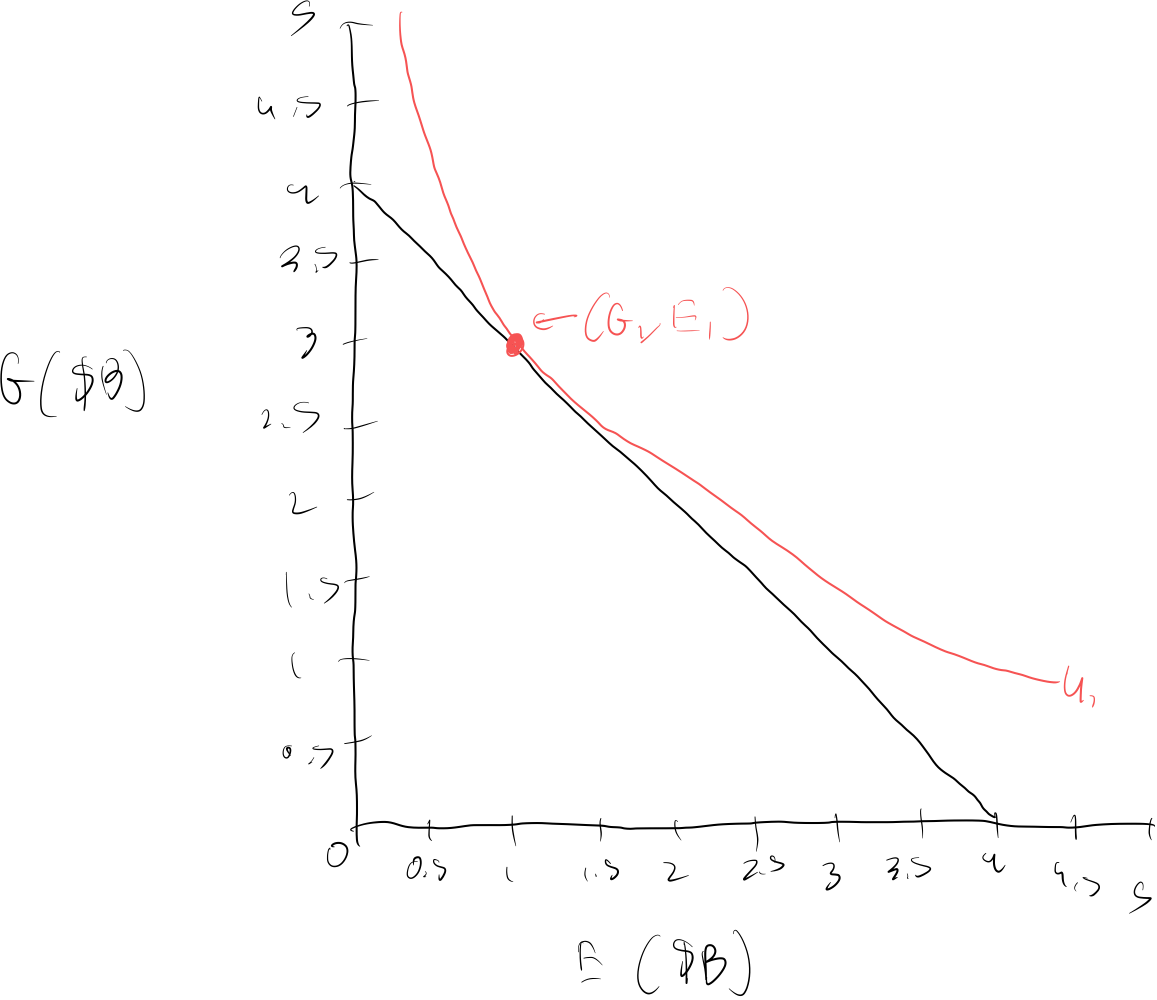
\includegraphics[width=0.5\textwidth]{images/3_4_a.png}
      \end{center}
    \end{problem}
    \begin{problem}{(b)}
      Solve mathematically for $E_1$.
      \tcblower
      \begin{align*}
        \shortintertext{Marginal Rate of Substitution}
        MRS_{GE_1} &= \frac{\frac{\partial U}{\partial G}}{\frac{\partial U}{\partial E}}\\
                   &= \frac{3E}{G}\\
                   \shortintertext{Set equal to price ratio}
        1 &= \frac{3E}{G}\\
        G &= 3E\\
        \shortintertext{Substitute into Budget Constraint}\\
        4 &= G + E \\
        4 &= 3E + E\\
        1 &= E_1
      \end{align*}
    \end{problem}
    Part of Delaware's new education strategy has been to give students access to top-notch, experienced teachers. But because most good teachers move to warmer states like Florida, Delaware has had to increase class sizes in order to achieve its strategy. The federal government is concerned that these larger class sizes are detrimental to educational achievement, and thus it has vowed to improve Delaware's education system. To figure out how best to do this, the US Department of Education has asked you to evaluate several proposals.

    \begin{description}
      \item[Federal Matching Grant] Suppose the federal government provides Delaware with a matching grant such that each \$1 of state spending on the education program is matched by \$1 from the federal government.
    \end{description}
    \begin{problem}{(c)}
      Present the state's revised problem graphically, as in part (a). Label the original and new budget constraints, the original and revised education spending, and the corresponding indifference curves at these choices.
      \tcblower
      \begin{center}
        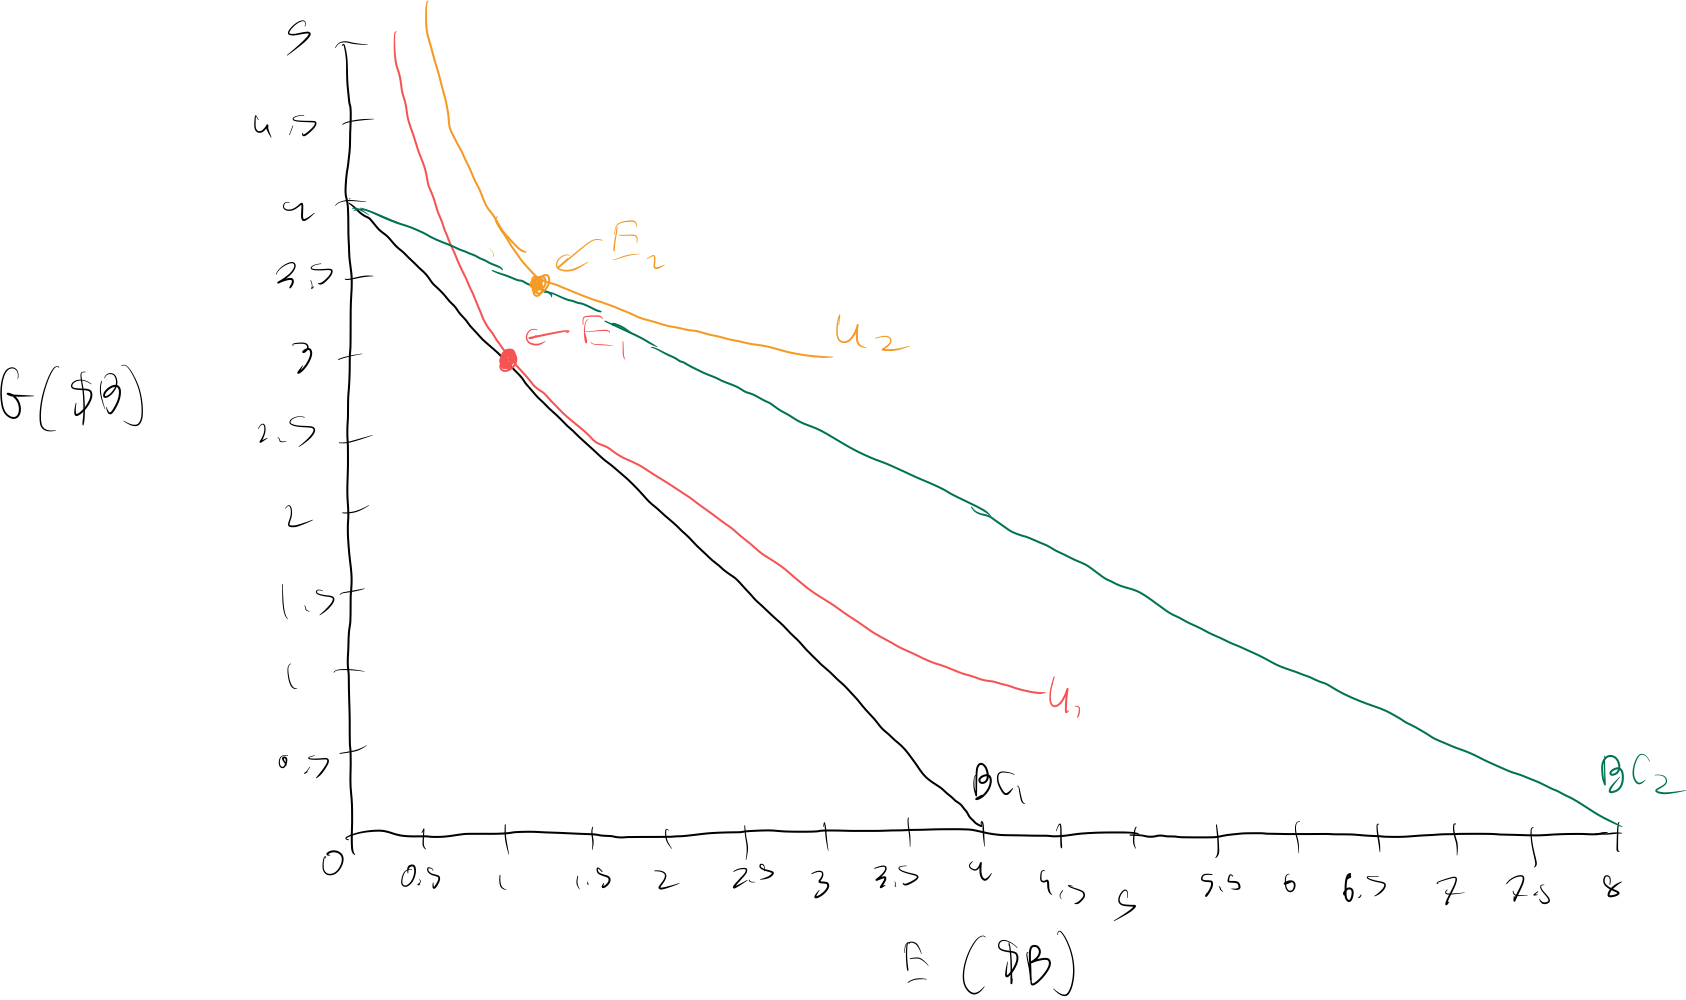
\includegraphics[width=0.5\textwidth]{images/3_4_c.png}
      \end{center}
    \end{problem}
    \begin{problem}{(d)}
      What is Delaware's effective price per unit of education under this proposal?
      \tcblower
      The effective price for Delaware is $\frac{1}{2}$ for a unit of educational quality, as to achieve one unit of educational quality, Delaware only needs to spend $\frac{1}{2}$ a unit (which is matched by $\frac{1}{2}$ a unit from the government)
    \end{problem}
    \begin{problem}{(e)}
      Solve mathematically for $E_2$.
      \tcblower
      \begin{align*}
        4 &= G +  \frac{1}{2}E \\
        8 &= 2G + E \\
        8 &= 7E \tag*{substitute $G = 3E$}\\
        E &= \frac{8}{7}
      \end{align*}
    \end{problem}
    \begin{problem}{(f)}
      How much money is the federal government giving to Delaware? Does the state contribute more, less, or the same amount to educational quality with this grant?
      \tcblower
      Since the total education spend is $\frac{8}{7}$, which is split 50-50, this means the government is spending $\frac{4}{7}$ and the state is spending $\frac{4}{7}$. The state contributes \textit{less} to educational quality with this grant.
    \end{problem}
    \begin{description}
      \item[Federal (Unconditional) Block Grant] Suppose instead that the federal government provides Delaware with a block grant of equivalent size to the federal grant calculated in part (f).
    \end{description}
    \begin{problem}{(g)}
      Present the state's revised problem graphically. Label the original and new budget constraints, the original and revised education spending, and the corresponding indifference curves.
      \tcblower
      \begin{center}
        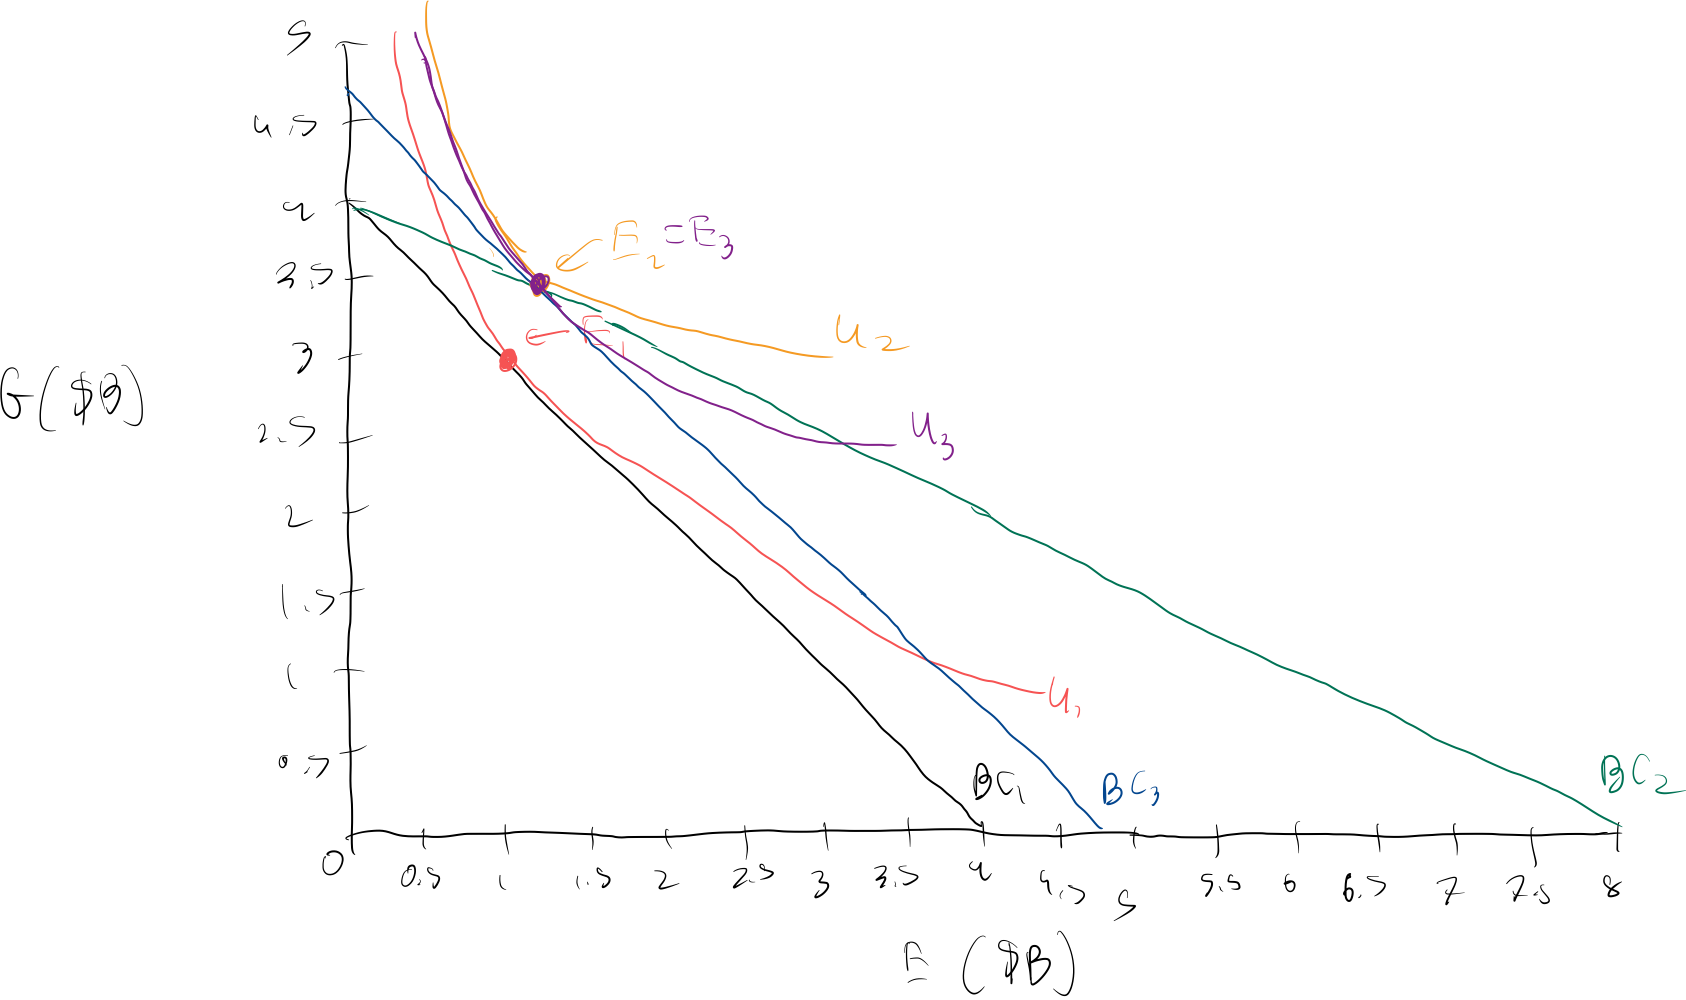
\includegraphics[width=0.5\textwidth]{images/3_4_g.png}
      \end{center}
    \end{problem}
    \begin{problem}{(h)}
      Solve mathematically for $E_3$.
      \tcblower
      \begin{align*}
        \frac{32}{7} &= G + E \\
      \frac{32}{7} &= 4E\\
      \frac{8}{7} &= E_3
      \end{align*}
    \end{problem}
    \begin{problem}{(i)}
      The size of the federal grant under this proposal is (by construction) the same as with the matching grant. Does the matching grant or block grant lead to higher educational quality? Explain your answer by discussing the role of income and substitution effects.
      \tcblower
      The matching and block grant, by construction, feature the same income effect; whereas the matching grant features a substitution effect toward spending on education, the block grant has no substitution effect.
    \end{problem}
    \begin{problem}{(j)}
      Assuming the validity of the behavioral ``flypaper effect,'' how would you expect the real world response of the block grant to compare with the theoretical prediction?
      \tcblower
      The real world response should see that education spend increases to $\frac{11}{7}$, rather than the $\frac{8}{7}$ that our model predicts.
    \end{problem}
    \begin{description}
      \item[Federal Conditional Block Grant] Suppose instead that the federal government provides Delaware with a conditional block grant of equivalent size to that calculated in (f), whereby the grant is provided to the state with a mandate that the grant be spent only on improving the quality of Delaware's education program.
    \end{description}
    \begin{problem}{(k)}
      How does this problem differ from the unconditional block grant? In particular, will the conditional block grant increase, decrease, or not change the level of education provided?
      \tcblower
      In the unconditional case, the $\frac{4}{7} $block grant could be spent on anything that the Delaware government desired, but in this case, the $\frac{4}{7}$ can only be spent on education. However, since $\frac{4}{7} < 1$, the conditional block grant will not change the level of education provided.
    \end{problem}
    \begin{problem}{(l)}
      If the federal government is specifically concerned with perceived under-provision of educational quality in Delaware, which intervention assessed above is most effective?
      \tcblower
      The matching grant is that which is most effective, as it reduces the price of provision of education on the part of the state.
    \end{problem}
    \begin{problem}{(m)}
      If the federal government is only concerned with the overall welfare, which intervention(s) assessed above would prove most effective?
      \tcblower
      The unconditional block grant would be the most effective at improving welfare for the median voter, as it leaves the relative level of education spending unchanged but improves overall income (and thus welfare).
    \end{problem}
  \end{problem}
\end{document}
